\chapter{Compiling Relay}
\label{ch:compiler}

\section{Background}
\label{sec:background}

% TODO: Jared broadly suggested cutting this section. We do need to remove a lot of content just to be
% under the page limit, so we should determine what, if anything, here needs to be kept. For example,
% is a broad introduction to deep learning really something a reader would expect? We could set up
% the problem of expressiveness and deployment in the intro and focus on what other frameworks fall
% short on and what we do differently.

In this section, we provide a brief background on contemporary deep learning,
  popular deep learning frameworks, and state-of-the-art
  models being developed.

\subsection{Deep Learning}

Deep learning (DL) has been used to achieve state-of-the-art results in applications ranging from
computer vision to game playing to natural language processing. Deep learning provides a collection of
techniques for learning functions that are difficult to program directly.

For example, suppose one wants to construct a function $f(x)$ to extract building addresses from
images of a street. One approach to writing $f(x)$ explicitly might be to write programs to identify
regions of the image that contain information pertinent to addresses (like street names or house
numbers), partition those regions into individual characters, and identify each character.
One may then write a program that chains together many such modules into a working system.
It would require hundreds, if not thousands, of human-hours of work and dozens of heuristics to
write any of those programs by hand, and there is no guarantee it will perform well.
By contrast, deep learning has, with relatively little code, been
used to approximate this entire recognition task with a single model. The learned system
outperforms all hand-crafted solutions \citep{streetview}.

A programmer solving a problem with DL performs three steps. First, she specifies a parametric
function (often called a \textit{model}, \textit{neural network}, or simply \textit{network})
$F(\theta, x)$ of the function that computes the desired value. She then \textit{trains} the model
by applying an optimization algorithm to find a set of parameters $\theta$ that results in an
acceptable approximation of the function on a collection of input-output pairs. Finally, she uses
her learned function to produce outputs for new inputs in a process called \textit{inference}.

In practice, DL engineers write procedural programs that manipulate \textit{tensors},
  multi-dimensional arrays of numbers.
These restrictions allow DL practitioners to take advantage of
  statistics, linear algebra, and real analysis.
In order to search for an assignment of parameters that produces a good approximation, we must first
  define what a ``good'' approximation of $f$ is and then find an algorithm that optimizes this metric.
The quality of an approximation is typically defined in terms of some ground truth to
  compare against $F(\theta, x)$.
This ground truth is usually provided in the form of a
\textit{training set}, a set of input-output pairs that has either been manually collected or
  extracted from an existing data set.
The function that scores the output of a network with respect
  to a ground-truth label is called the \textit{loss function},
\[
  L \colon (\text{input}, \text{output}) \to \text{network} \to \mathbb{R}^{\ge 0},
\]
which typically takes in an input-output pair and network and produces a non-negative real
number.

One method to optimize the network is to take the gradient of the loss function composed with the
candidate network for some input-output pair. The gradient of a function points in the direction of
steepest change, so subtracting some proportion of the gradient from the current parameters reduces
the loss of the network. This process is known as \textit{stochastic gradient descent (SGD)}, and it
is the basis for many deep learning optimization algorithms used today.

More formally, training updates the model parameters using the following algorithm:
\[
  \theta_{i+1} := \theta_i - \varepsilon\nabla[L((\text{input}, \text{output})) \circ F]\Big|_{\theta_i}
\]
for some small, positive $\varepsilon$. This update cycle is repeated in training until
the error is acceptable. The final values of the parameters are then used for inference.

While training and inference were once performed on the same machine, it is more common today to
train models on high-powered devices such as a fleet of cloud machines or a custom GPU farm, since
training is very computationally intensive. The values learned from training can then be deployed
for inference on less powerful systems, such as a single GPU, a mobile phone, or an FPGA.

\subsection{Deep Learning Framework Design and Limitations}

Popular deep learning frameworks began with designs
  optimized for different tradeoffs between
  expressivity, performance, and portability.
In the early days of deep learning, users would program
  in general purpose languages like Python and utilize
  scientific computing libraries like NumPy,
  which provides low-level \textit{operators} such as matrix multiplication.
Operators, also called kernels, are dense linear algebra primitives like matrix multiplication,
  elementwise functions like \verb|tanh|,
  and complex, domain-specific operations like image convolution.
Operator execution dominates the execution time of a deep learning model: many
  operators are asymptotically slow and their input is often large.
While a machine learning framework may be written as a library in a high-level language
  like Python or Swift, operators will typically be provided as opaque function calls to
  specialized implementations written in a lower-level language like C++.

In order to obtain better performance, researchers began utilizing specialized accelerators.
To expose accelerators to end-users without needing to write in low-level languages,
such as CUDA, researchers designed frameworks like Theano~\citep{theano}.
These frameworks represent computations using dataflow graphs
  (treating mathematical operations on data as nodes)
  and compile these graphs to deploy to
  accelerators like the GPU.
``Computation graphs'' provide a limited programming model,
  enabling efficient deployment.
Computation graphs have since been adopted as the fundamental building block of modern
  machine learning libraries.

There are two dominant designs for computation graph-based frameworks.
The first is the declarative design employed by TensorFlow.
Such designs extend pure data-flow with \textit{ad hoc} control operations
  to emulate the functionality of \verb|if| and \verb|while|.
This approach is called \textit{define-then-run} and employs \textit{static
computation graphs}.
A framework using a define-then-run representation has access to the entire
  graph before execution, providing more opportunities to optimize the program
  as well as simplifying deployment since the program can be executed
  without the host language.
However, the control flow structures are less expressive than those supported
  by the host language, frustrating researchers who wish to experiment with complex models.
For example, TensorFlow supports loops,
  but the elaborated graph has little resemblance to the input program, requiring optimization
  authors to reason about the elaborated form instead of familiar loops.
The encoding also requires \textit{ad hoc}, special purpose operators such
  as \verb|NextIteration| and the addition of special control-edges to the graph.
There are no generic mechanisms for users to define new control flow
  combinators (e.g., \verb|fold|) or data types.

The second approach is used by PyTorch, where the host language (e.g. Python) dynamically
  constructs a computation graph.
This approach is called \textit{define-by-run} and employs \textit{dynamic computation graphs}.
An arbitrary host program executes dynamically, generating a computation graph as a by-product,
  allowing for use of all host language features.
However, by not encoding control constructs in its IR, a framework
  using define-by-run cannot reason about or optimize control flow structures.
Not only does this leave performance on the table, but it prevents deployment to certain
  edge devices, since they may have control flow or memory requirements that cannot be
  guaranteed by a fully dynamic control plane.

\subsection{Dynamic Neural Networks}

One area in which deep learning has made significant advances is
  natural language processing (NLP), such as finding keywords in a
  research paper, determining the sentiment of a tweet,
  or summarizing a news article.
Reasoning about text requires context-sensitive analysis and data of
  non-fixed dimensions, unlike in many vision tasks.
To allow for context-sensitive analysis, DL researchers have developed networks with persistent
state, known as \textit{recurrent neural networks}  (RNNs). Like the simple networks described
earlier, these networks have an input and an output; however, they take an additional input and
produce an additional output known as the \textit{hidden state}. Beginning with an initial hidden
state and a list of inputs (for example, characters from a source text), one can produce a
list of outputs (for example, a translation of the source text). %, as in Fig.~\ref{fig:rnn_graph}.
Recurrent neural networks have found use not only in NLP, but also in speech recognition, music
transcription, eSports, and other areas \citep{lstm, speech_recognition, OpenAI_dota}.

Unfortunately, since most machine learning frameworks rely on computation graphs,
  which cannot represent recursion, RNNs are usually finitely unrolled to a fixed depth.
This may be acceptable if the depth can be determined statically and the loop unrolled
  ahead of time; however, if the depth depends on runtime values or complex control flow,
  unrolling must be performed dynamically.
% Since the source language is usually an interpreted language like Python, this process incurs significant
% overhead. Even when unrolling can be computed ahead of time, it destroys information about
% the original program, which can no longer be used for ahead-of-time optimization.

\subsection{Hardware Backends}

If a programmer wants to experiment with a new hardware device,
  she must manually account for variations in hardware intrinsics, data
  types, and data layout.
This is only possible if the device is supported by her framework of choice.
Even with the addition of device-specific code,
  there is no guarantee performance will be acceptable, let alone optimal
  (or even that there will not be regression).
Many existing IRs also do not support data-dependent control flow.
If she cannot capture her model (e.g., an RNN) in the IR,
  she cannot deploy to hardware backends without requiring a host to drive
  execution.
In order to effectively use these devices,
  engineers often redesign the model from scratch to better match the target
  platform's intrinsics and design.

% \begin{figure}[!h]
%   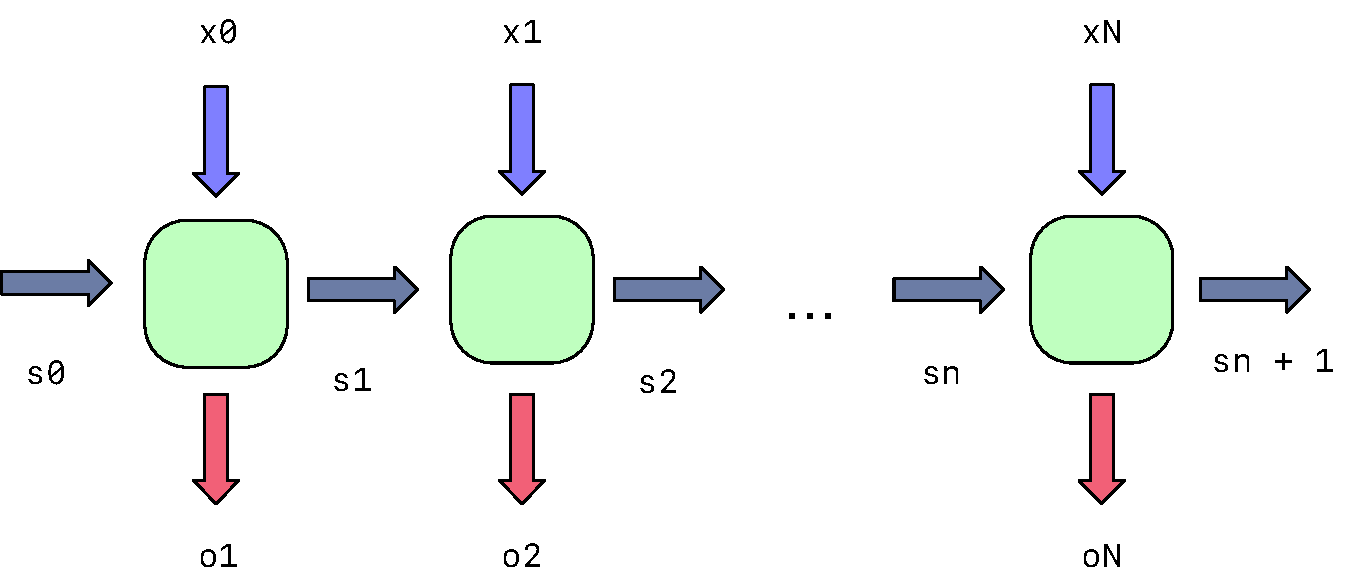
\includegraphics[width=0.9\columnwidth, height=5cm]{fig/rnn_graph}
%   \caption{
%     An RNN unrolled to time step $N$. The input arrows prefixed with $x$ are inputs,
%     the horizontal arrows prefixed $s$ are the hidden states, and the output arrows
%     are positional outputs of the model. For example each output would be a single
%     character of the names we generate in Section \ref{sec:overview}.}
%   \label{fig:rnn_graph}
% \end{figure}


% % For example,
% %   convolutional neural networks (CNNs),
% %   which are widely used in image processing and computer vision,
% %   generally utilize a fixed topology of layers
% %   with tensors of fixed dimension.
% % In contrast,
% %   recurrent neural networks (RNNs),
% %   which are widely used in natural language processing (NLP),
% %   require recursion, control flow, and
% %   operations over variable-sized data structures (e.g., lists).
% % The regular structure of CNNs facilitates
% %   optimizing compilation to
% %   common hardware accelerators (e.g., GPUs), but
% %   RNN-like models are still challenging to optimize.

% % INTEGRATE ME (DONE)

% % INTEGRATE ME PART 2
% % \subsection{Expressivity}
% % Most frameworks have employed a computation graph based IR.
% % These existing IRs are limited by their lack of flexibility as
% %   a programming language.
% % \todo{make this more crisp}
% % At first computation graphs appear to provide a compelling story for deployment to multiple devices.
% % Their emphasis on data flow makes it easy to port to new platforms, since one only has to think
% % about operators.

% % A limited programming model is both a strength and weakness,
% %   restricted semantics gives rise to efficient execution and
% %   straightforward portability.
% % Execution of a pure data-flow graph is well studied, and portability
% %   is determined by whether the platform has operator support.
% % Unfortunately the IR limits the set of programs that can be
% %   represented, recursive models such as RNNs and LSTMs
% %   can not be directly encoded and must be unrolled.
% % In order to grow the set of programs that can be represented,
% %   existing IRs have added numerous ad-hoc extensions.
% % For example, TensorFlow requires a complex
% %   encoding to support loops, and specialized containers such
% %   as TensorArray to support loop accumulation.
% % These extensions are enough to capture a set of
% %   useful models, but limit future extensibility.
% % For example there are no generic mechanisms for users
% %   to define new control flow combinators (e.g., \verb|fold|) or data types.
%   % ~\citep{
%   %   tf_fold, tangent, tf_eager, xla, glow, pytorch_caffe2}.
% % The deep learning community has seen multiple iterations
% %   of popular model architectures, and there
% %   is strong evidence user's needs will continue
% %   to evolve.

% \jmp{missing a so what here. imo it should be moved out of this section or cut entirely}
% New model architectures, such as the transformer, continue to
%   emerge, and the essential set of models, which demand
%   the best performance, continues to rapidly change.
% The transformer architecture itself is not yet two years
%   old, with multiple improvements published in just the past year.
% \todo{cites}
% A quickly evolving landscape requires frameworks,
%   and by extension their compilers, to adapt to emerging applications.

% % \subsection{Performance}
% \jmp{missing a so what for this paragraph}
% Even if a model can execute on
%   a particular hardware device, developers
%   often manually design model
%   variants for each target platform
%   to achieve the best performance.
% Engineers design these platform specific model variants
%   through tedious experimentation and framework-specific tweaks
%   to achieve acceptable performance~\citep{mobilenet, xnor_net, squeezenet}.
% For example,
%   engineers may need to \textit{quantize} models
%   by manually reducing numerical precision for a particular platform,
%   sacrificing some accuracy for better performance~\citep{xnor_net}.
% Manually tuning models requires
%   that engineers learn the details of
%   each platform's
%   unique data types, intrinsics, and memory systems~\citep{fb_fp_hw, tpuv1, brainwave, nn_on_si}.

% While a small number of transformations have been automated, they often lack flexibility and
% composibility. Consider quantization, the transformation that replaces floating point numbers with
% lower-precision fixed point numbers to trade model accuracy for speed and size. This transformation
% has been automated in TensorFlow with TensorFlow Lite~\citep{tflite}. To convert a TensorFlow model
% to a TensorFlow Lite model, a developer either runs quantization-aware training or converts a model
% directly to TensorFlow Lite. In either case, the bulk of the work is done by a translation from a
% TensorFlow computation graph to a TensorFlow Lite computation graph with 8-bit quantized operators.

% Although the TensorFlow Lite pass is straightforward, its design limits its extensibility. It does
% not allow for different or mixed precisions, let alone different quantization strategies.
% Furthermore, rather than using quantization like any other optimization, a developer must run a
% special converter to transform their TensorFlow computation graph into a quantized TensorFlow Lite
% computation graph, (presumably) precluding the use of TensorFlow optimizations on the quantized
% model.
% % TODO: cite https://www.tensorflow.org/lite/guide#tensorflow_lite_architecture and maybe some other
% % stuff, too

% TensorFlow Lite also rewrites much of the TensorFlow runtime system as well as bakes in 8-bit
% quantized operators. To gain full extensibility, operations would have to be written for every
% precision-platform pair.

% % \jmp{it's still not clear \textit{what} about existing frameworks prevents them from doing better}

% % A limited number of these transformations such as quantization have
%   % become automated, but are often inflexible and non-composable.
% % The rigidity of these passes are in contrast traditional
% %   compiler passes which are designed for composition.
% % Non-composable passes make it impossible for users to mix and
% %   match optimizations to suit their application needs, including
% %   integrating new optimizations.

% % \subsection{Portability}
% % \jmp{needs a topic sentence}
% % To further complicate matters the number of hardware platforms
% %   for deep learning is growing rapidly.
% % Beyond deploying machine learning in traditional services,
% %   developers may now train models in the
% %   cloud and deploy them to edge devices, such as mobile phones.
% % Many deployment targets, such as mobile phones, are a heterogenous system
% %   consisting of a CPU, GPU, and customized machine learning accelerator.
% % The number of specialized hardware
% %   accelerators available is rapidly growing~\citep{moreau2018vta, OpenTPU, tpuv1}.
% % Accelerators provide an attractive way to decrease
% %   the execution time, memory and power consumption of models while
% %   increasing the number of contexts deep learning can be deployed in.

% % Obtaining optimal performance from accelerators, requires
% %   mapping high-level computation to a device's limited
% %   instruction set.
% % Frameworks are often not designed for this use case \jmp{why not?} resulting in brittle
% %   software stack with support for a limited number of models.
% % Targeting accelerators requires sophisticated compilers which
% %   must perform a variety of optimizations and schedule computation across
% %   heterogenous devices.
% %   \todo{cite here, ask luis}
% % It is essential that frameworks can adapt to new hardware devices
% %   with minimal changes to applications.

Transforming Relay into code that executes efficiently on a variety of networks requires a series of transformations, and must interact with TVM and other layers below it.
